\section{Рэалізацыя канвеера бесперапыннай інтэграцыі і дастаўкі}

У дадзеным раздзеле будзе разгледжаны прыклад рэалізацыі
канвеера бесперапыннай інтэграцыі і дастаўкі пры дапамозе
open-source рашэнняў[\ref{site:CI/CD-pipeline}].

\subsection{Пастаноўка задачы}

Неабходна распрацаваць канвеер бесперапыннай інтэграцыі і дастаўкі
для Web-праграмы, якая напісаная на мове праграмавання Python.
У канвееры неабходна настроіць выкананне аўтаматызаваных тэстаў і
пастаянную праверку якасці кода.
Запуск праграмы мае ажыццяўляцца ўнутры Docker-кантэйнера.

\subsection{Праграма генератара фраз}

Створым невялікую кансольную праграму, якая будзе генерыраваць
фразы. Зыходны код прадстаўлены ў лістынгу \ref{lst:generator.py}:
\lstinputlisting[caption={Зыходны код праграмы generator.py},%
                            label={lst:generator.py},%
                            language=Python]{generator.py}

На малюнку \ref{figure:output of generator.py} прадстаўлены вывад
праграмы generator.py, дзе можаш пераканацца ў тым, што пры кожным
запуску вывад праграмы адрозніваецца.

\clearpage

\begin{figure}[h!]
    \centering
    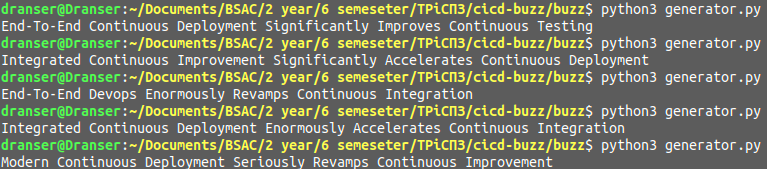
\includegraphics[width=\textwidth]{output_of_generator_py}
    \caption{Вывад праграмы generator.py}
    \label{figure:output of generator.py} 
\end{figure}

\vspace{-\baselineskip}
\subsection{Аўтаматызаваныя тэсты}

Створым некалькі unit-тэстаў для праверкі працаздольнасці праграмы.
Зыходны код unit-тэстаў прадстаўлены ў лістынгу
\ref{lst:test_generator.py}:

\lstinputlisting[caption={Зыходны код праграмы test\_generator.py},%
                            label={lst:test_generator.py},%
                            language=Python]{test_generator.py}

Unit-тэсты будуць запускацца пры дапамозе фрэймфворка "pytest".
Вывад запуску unit-тэстаў прадстаўлены на малюнку
\ref{figure:output of test_generator.py}.

\clearpage

\begin{figure}[h!]
    \centering
    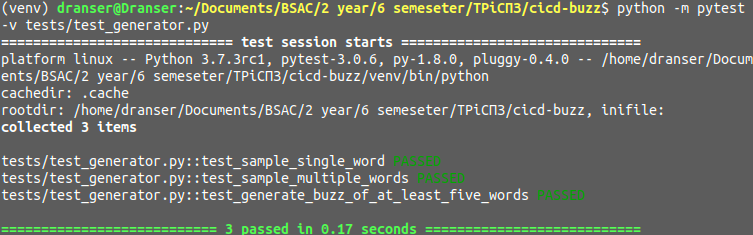
\includegraphics[width=\textwidth]{output_of_test_generator_py}
    \caption{Вывад праграмы test\_generator.py}
    \label{figure:output of test_generator.py} 
\end{figure}

На малюнку \ref{figure:output of test_generator.py} можам бачыць,
што праграма generator.py паспяхова прайшла ўсе unit-тэсты.

\subsection{Выкананне тэстаў пры дапамозе Travis CI}

Для выканання тэстаў у аўтаматычным рэжыме пры кожным змяненні
кода на GitHub неабходна падключыць для дадзенага рэпазіторыя
сервіс Travis CI і паставіць настройкі для выканання зборкі пры
кожным push альбо pull запыце рэпазіторыя
(малюнак \ref{figure:setting of Travis CI}).

\begin{figure}[h!]
    \centering
    
\includegraphics[width=\textwidth]{setting_of_Travis_CI}
    \caption{Настройка зборкі пры push- і pull-запытах у Travis CI}
    \label{figure:setting of Travis CI} 
\end{figure}

Апошні крок для актывацыі Travis CI заключаецца ў дабаўленні файла
канфігурацыі ".travis.yml", змест каторага прадстаўлены ў лістынгу
\ref{lst:travis_yml}.

\lstinputlisting[caption={Канфігурацыя Travis CI},%
                            label={lst:travis_yml}]{travis.yml}

Цяпер пры кожным push- альбо pull-запыце да рэпазіторыя на GitHub
у аўтаматычным рэжыме будуць запускацца unit-тэсты на сервісе Travis CI.
Рэзультаты unit-тэстаў можна праглядаць у кансолі Travis CI
(малюнак \ref{figure:output of Travis CI}).

\clearpage

\begin{figure}[h!]
    \centering
    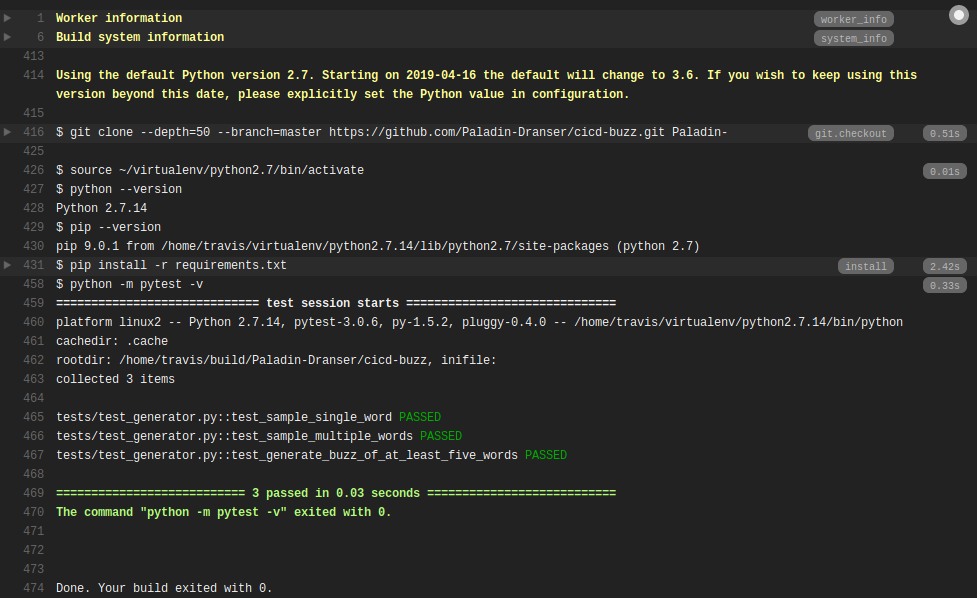
\includegraphics[width=\textwidth]{output_of_Travis_CI}
    \caption{Вывад рэзультатаў праходжання unit-тэстаў
             у кансолі Travis CI}
    \label{figure:output of Travis CI} 
\end{figure}

\vspace{-\baselineskip}
\subsection{Праверка якасці кода пры дапамозе Better Code Hub}

Інтэграцыя сервісa Better Code Hub да рэпазіторыя на GitHub
дазваляе аналізаваць якасць кода пры кожным push- і pull-запыце
(падобна сервісу Travis CI).

Вынік праверкі якасці кода прадстаўлены на малюнку
\ref{figure:Better Code Hub}, на якім можам бачыць,
што код адпавядае ўсім неабходным патрабаванням.


\begin{figure}[h!]
    \centering
    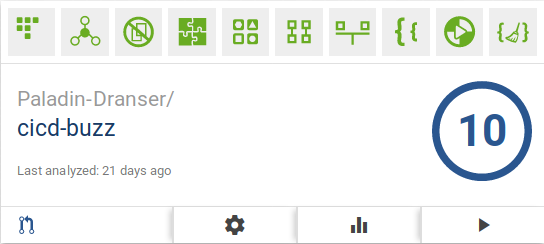
\includegraphics[width=0.8\textwidth]{better_of_code_hub}
    \caption{Вынік праверкі якасці кода пры дапамозе Better Code Hub}
    \label{figure:Better Code Hub} 
\end{figure}

\subsection{Web-праграма для генерацыі фраз}

Згодна з пастаўленай задачай ператворым нашу кансольную праграму
генерацыі фраз ў Web-праграму.

Для гэтага створым новую праграмы з выкарыстаннем фрэймворка Flask,
якая будзе выкарыстоўваць раней напісаны модуль generator.py.

Зыходны код праграмы прадстаўлены ў лістынгу \ref{lst:app.py}:

\lstinputlisting[caption={Зыходны код Web-праграмы app.py},%
                            label={lst:app.py},%
                            language=Python]{app.py}

Вынік Web-праграмы прадстаўлены на малюнку \ref{figure:Web application}.

\begin{figure}[h!]
    \centering
    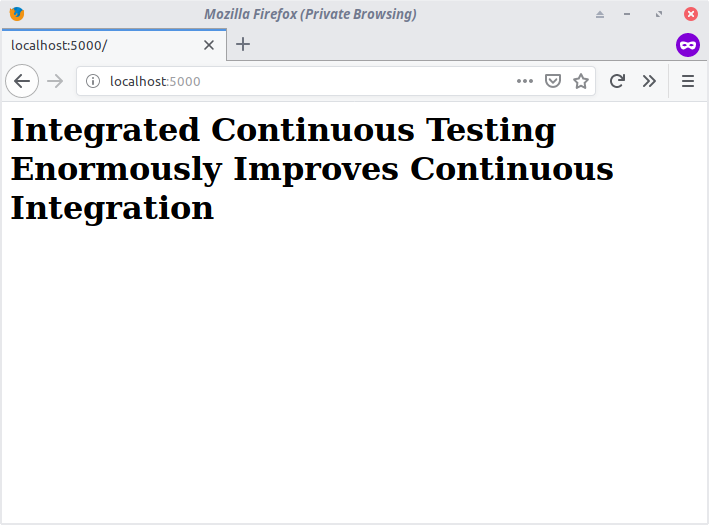
\includegraphics[width=0.6\textwidth]{web_application}
    \caption{Вынік Web-праграмы генерацыі фраз}
    \label{figure:Web application} 
\end{figure}

\subsection{Кантэйнерызацыя праграмы пры дапамозе Docker}

Адпаведна пастаўленай задачы рэалізуем Docker-кантэйнер
(пры дапамозе Dockerfile) для Web-праграмы.

Канфігурацыя Dockerfile прадстаўлена ў лістынгу \ref{lst:Dockerfile}.

\lstinputlisting[caption={Канфігурацыя Docker-кантэйнера},%
                 label={lst:Dockerfile}]{Dockerfile.txt}

Згодна з канфігурацыяй Docker загрузіць вобраз alpine,
установіць Python, pip, неабходныя кампаненты для запуску праграмы,
Web-праграму.
Web-праграма будзе запускацца пры запуску кантэйнера.

Такім чынам мы атрымалі Web-праграму, якая запускаецца ўнутры кантэйнера
і не залежыць ад знешніх канфігурацый асяроддзя.
Пры змяненні зыходнага кода праграмы альбо канфігурацый сервісаў
адбываецца аўтаматычная зборка і тэсціраванне праграмы.
